% LaTeXar con :
%  pdflatex eldiego.tex
%"The PDF file may contain up to 25 pages of reference material, single-sided, letter or A4 size, with text and illustrations readable by a person with correctable eyesight without magnification from a distance of 1/2 meter."
\documentclass[10pt,landscape,twocolumn,a4paper,notitlepage]{article}
\usepackage{hyperref}
\usepackage[spanish, activeacute]{babel}
\usepackage[utf8]{inputenc}
\usepackage{fancyhdr}
\usepackage{lastpage}
\usepackage{listings}
\usepackage{amssymb}
\usepackage[usenames,dvipsnames]{color}
\usepackage{graphicx}
\usepackage{wrapfig}



%%% Margenes
\setlength{\columnsep}{0.25in}    % default=10pt
\setlength{\columnseprule}{0.5pt}    % default=0pt (no line)
 
\addtolength{\textheight}{2.35in}
\addtolength{\topmargin}{-0.9in}     % ~ -0.5 del incremento anterior
 
\addtolength{\textwidth}{1.1in}
\addtolength{\oddsidemargin}{-0.55in} % -0.5 del incremento anterior
 
\setlength{\headsep}{0.08in}
\setlength{\parskip}{0in}
\setlength{\headheight}{15pt}
\setlength{\parindent}{0mm}
 
%%% Encabezado y pie de pagina
\pagestyle{fancy}
\fancyhead[LO]{\textbf{\title}}
\fancyhead[C]{\leftmark\ -\ \rightmark}
\fancyhead[RO]{P\'agina \thepage\ de \pageref{LastPage}}
\renewcommand{\headrulewidth}{0.4pt}
\fancyfoot{}
\definecolor{darkblue}{rgb}{0,0,0.4}
%%% Configuracion de Listings
\lstloadlanguages{C++}
\lstnewenvironment{code}
	{%\lstset{	numbers=none, frame=lines, basicstyle=\small\ttfamily, }%
	 \csname lst@SetFirstLabel\endcsname}
	{\csname lst@SaveFirstLabel\endcsname}
\lstset{% general command to set parameter(s)
	language=C++, basicstyle=\small\ttfamily, keywordstyle=\slshape,
	emph=[1]{tipo,usa}, emphstyle={[1]\sffamily\bfseries},
	morekeywords={tint,forn,forsn},
	basewidth={0.47em,0.40em},
	columns=fixed, fontadjust, resetmargins, xrightmargin=5pt, xleftmargin=15pt,
	flexiblecolumns=false, tabsize=2, breaklines,	breakatwhitespace=false, extendedchars=true,
	numbers=left, numberstyle=\tiny, stepnumber=1, numbersep=9pt,
	frame=l, framesep=3pt,
    basicstyle=\ttfamily,
    keywordstyle=\color{darkblue}\ttfamily,
    stringstyle=\color{magenta}\ttfamily,
    commentstyle=\color{RedOrange}\ttfamily,
    morecomment=[l][\color{OliveGreen}]{\#}
}

\lstdefinestyle{C++}{
	language=C++, basicstyle=\small\ttfamily, keywordstyle=\slshape,
	emph=[1]{tipo,usa,tipo2}, emphstyle={[1]\sffamily\bfseries},
	morekeywords={tint,forn,forsn},
	basewidth={0.47em,0.40em},
	columns=fixed, fontadjust, resetmargins, xrightmargin=5pt, xleftmargin=15pt,
	flexiblecolumns=false, tabsize=2, breaklines,	breakatwhitespace=false, extendedchars=true,
	numbers=left, numberstyle=\tiny, stepnumber=1, numbersep=9pt,
	frame=l, framesep=3pt,
    basicstyle=\ttfamily,
    keywordstyle=\color{darkblue}\ttfamily,
    stringstyle=\color{magenta}\ttfamily,
    commentstyle=\color{RedOrange}\ttfamily,
    morecomment=[l][\color{OliveGreen}]{\#}
}
 
%%% Macros
\def\nbtitle#1{\begin{Large}\begin{center}\textbf{#1}\end{center}\end{Large}}
\def\nbsection#1{\section{#1}}
\def\nbsubsection#1{\subsection{#1}}
\def\nbcoment#1{\begin{small}\textbf{#1}\end{small}}
\newcommand{\comb}[2]{\left( \begin{array}{c} #1 \\ #2 \end{array}\right)}
\def\complexity#1{\texorpdfstring{$\mathcal{O}(#1)$}{O(#1)}}
 \newcommand\cppfile[2][]{
\lstinputlisting[style=C++,linerange={#1}]{#2}
}

\begin{document}
\def\title{El Diego 2.0}
\centering{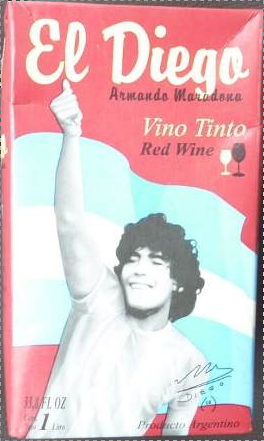
\includegraphics[width=4cm]{fotodiego}}
\tableofcontents\newpage

 
\section{algorithm}%%%%%%%%%%%%%%%%%%ALGORITHM%%%%%%%%%%%%%%%%%%
\textbf{\#include $<$algorithm$>$ \#include $<$numeric$>$ \\}
\begin{tabular}{|l|l|p{5.4cm}|} \hline
\textbf{Algo} & \textbf{Params} &  \textbf{Funcion} \\  \hline
%swap & e1, e2 &  da vuelta e1,e2 & $1$\\\hline
sort, stable\_sort & f, l &  ordena el intervalo \\  \hline
%is\_sorted & f, l &  \textit{bool} si esta ordenado \\  \hline
nth\_element & f, nth, l & \textit{void} ordena el n-esimo, y \\ && particiona el resto \\  \hline
fill, fill\_n & f, l / n, elem & \textit{void} llena [f, l) o [f, \\ && f+n) con elem \\  \hline
lower\_bound, upper\_bound & f, l, elem & \textit{it} al primer / ultimo donde se \\ && puede insertar elem para que\\ && quede ordenada \\  \hline
binary\_search & f, l, elem & \textit{bool} esta elem en [f, l) \\  \hline
copy & f, l, resul & hace resul+$i$=f+$i$ $\forall i$ \\  \hline
find, find\_if, find\_first\_of & f, l, elem & \textit{it} encuentra i $\in$[f,l) tq. i$=$elem, \\ & / pred / f2, l2 & pred(i), i$\in$[f2,l2)\\\hline
count, count\_if & f, l, elem/pred & cuenta elem, pred(i)\\\hline
search & f, l, f2, l2 & busca [f2,l2) $\in$ [f,l)\\\hline
replace, replace\_if & f, l, old & cambia old / pred(i) por new \\ & / pred, new &\\\hline
reverse & f, l & da vuelta\\\hline
partition, stable\_partition & f, l, pred & pred(i) ad, !pred(i) atras\\\hline
%min, max & e1, e2 & men / may & $1$\\\hline
min\_element, max\_element & f, l, [comp] & \textit{it} min, max de [f,l]\\\hline
lexicographical\_compare & f1,l1,f2,l2 & \textit{bool} con [f1,l1]<[f2,l2]\\\hline
next/prev\_permutation & f,l & deja en [f,l) la perm sig, ant\\\hline
set\_intersection, & f1, l1, f2, l2, res & [res, $\ldots$) la op. de conj\\
set\_difference, set\_union, & & \\
set\_symmetric\_difference, & &\\\hline
push\_heap, pop\_heap, & f, l, e / e / & mete/saca e en heap [f,l), \\
make\_heap & & hace un heap de [f,l)\\\hline
is\_heap & f,l & \textit{bool} es [f,l) un heap\\\hline
accumulate & f,l,i,[op] & \textit{T} $=$ $\sum$/oper de [f,l)\\\hline
inner\_product & f1, l1, f2, i & \textit{T} $=$ i $+$ [f1, l1) . [f2, $\ldots$ )\\\hline
partial\_sum & f, l, r, [op] & r+i = $\sum$/oper de [f,f+i] $\forall i \in$[f,l)\\\hline
%power & e, i, op & \textit{T} = $e^{n}$\\\hline
\_\_builtin\_ffs& unsigned int & Pos. del primer 1 desde la derecha\\\hline
\_\_builtin\_clz & unsigned int & Cant. de ceros desde la izquierda.\\\hline
\_\_builtin\_ctz & unsigned int & Cant. de ceros desde la derecha.\\\hline
\_\_builtin\_popcount & unsigned int & Cant. de 1’s en x.\\\hline
\_\_builtin\_parity & unsigned int & 1 si x es par, 0 si es impar.\\\hline
\_\_builtin\_llXXXXXX & unsigned ll & = pero para long long's.\\\hline
\end{tabular}



\section{Estructuras}%%%%%%%%%%%%%%%%%%ESTRUCTURAS%%%%%%%%%%%%%%%%%%
\subsection{RMQ (static)}
Dado un arreglo y una operación asociativa \emph{idempotente}, get(i, j) opera sobre el rango [i, j). Restricción: LVL $\ge$ ceil(logn); Usar [ ] para llenar arreglo y luego build().
\cppfile{estructuras/rmq.static.cpp}
\subsection{RMQ (dynamic)}
\cppfile{estructuras/rmq.dynamic.cpp}
\subsection{RMQ (lazy)}
\cppfile{estructuras/rmq.lazy.cpp}
\subsection{Fenwick Tree}
\cppfile{estructuras/fenwick.cpp}
\subsection{Union Find}
\cppfile{estructuras/union.find.cpp}
\subsection{Disjoint Intervals}
\cppfile{estructuras/disjoint.intervals.cpp}
\subsection{RMQ (2D)}
\cppfile{estructuras/rmq.2d.cpp}
\subsection{Big Int}
\cppfile{estructuras/bigint.cpp}
\subsection{Modnum}
\cppfile{estructuras/mnum.cpp}
\subsection{Treap}
\cppfile[4-99]{estructuras/treap.cpp}
\subsection{Bittrie}
\cppfile{estructuras/bitrie.cpp}


\section{Strings}%%%%%%%%%%%%%%%%%%STRINGS%%%%%%%%%%%%%%%%%%%%%%%%%%
\subsection{KMP}
\cppfile[21-43]{string/kmp.cpp}
\subsection{Trie}
\cppfile{string/trie.cpp}
\subsection{Suffix Array (corto, nlog2n)}
\cppfile[12-26]{string/suffix.array.short.cpp}
\subsection{Suffix Array (largo, nlogn)}
\cppfile[-34]{string/suffix.array.cpp}
\subsection{String Matching With Suffix Array}
\cppfile[37-58]{string/suffix.array.cpp}
\subsection{LCP (Longest Common Prefix)}
\cppfile[60-75]{string/suffix.array.cpp}
\subsection{Corasick}
\cppfile[9-51]{string/corasick.cpp}


\section{Geometría}%%%%%%%%%%%%%%%%%%GEOMETRIA%%%%%%%%%%%%%%%%%%%%%%
\#define EPS 1e-9
\subsection{Punto}
\cppfile{geometria/pto.cpp}
\subsection{Line}
\cppfile{geometria/line.cpp}
\subsection{Segment}
\cppfile{geometria/segm.cpp}
\subsection{Rectangle}
\cppfile{geometria/rect.cpp}
\subsection{Polygon Area}
\cppfile{geometria/area.cpp}
\subsection{Circle}
\cppfile{geometria/circle.cpp}
\subsection{Point in Poly}
\cppfile{geometria/point.in.poly.cpp}
\subsection{Convex Check CHECK}
\cppfile{geometria/convex.check.cpp}
\subsection{Convex Hull}
\cppfile{geometria/convex.hull.cpp}
\subsection{Cut Polygon}
\cppfile{geometria/cut.polygon.cpp}
\subsection{Bresenham}
\cppfile{geometria/bresenham.cpp}
\subsection{Rotate Matrix}
\cppfile{geometria/rotate.cpp}


\section{Math}%%%%%%%%%%%%%%%%%%MATH%%%%%%%%%%%%%%%%%%%%%%%%%%%%%%%%
\subsection{Combinatorio}
\cppfile{math/combinatorio.cpp}
\subsection{Exp. de Matrices en log(n)}
\cppfile{math/exp.mat.cpp}
\subsection{Phollard's Rho}
\cppfile[8-36]{math/phollards.rho.cpp}
\subsection{Criba}
\cppfile[20-30]{math/criba.cpp}
\subsection{Factorizacion}
Sea $n=\prod{p_i^{k_i}}$, fact(n) genera un map donde a cada $p_i$ le asocia su $k_i$
\cppfile[31-42]{math/factorizacion.cpp}
\subsection{GCD}
\begin{code}
tipo gcd(tipo a, tipo b){return a?gcd(b %a, a):b;}
\end{code}
\subsection{LCM}
\begin{code}
tipo lcm(tipo a, tipo b){return a / gcd(a,b) * b;}
\end{code}
\subsection{Simpson}
\cppfile{math/simpson.cpp}
\subsection{Fraction}
\cppfile{math/frac.cpp}
\subsection{Polinomio}
\cppfile{math/polinomio.cpp}


\section{Grafos}%%%%%%%%%%%%%%%%%%GRAFOS%%%%%%%%%%%%%%%%%%%%%%%%%%%%
\subsection{Dijkstra}
\cppfile{grafos/dijkstra.cpp}
\subsection{Bellman-Ford}
\cppfile{grafos/bellman.ford.cpp}
\subsection{Floyd-Warshall}
\cppfile{grafos/floyd.warshall.cpp}
\subsection{Kruskal}
\cppfile[27-41]{grafos/kruskal.cpp}
\subsection{Prim}
\cppfile[23-40]{grafos/prim.cpp}
\subsection{2-SAT + Tarjan SCC}
\cppfile{grafos/2sat.cpp}
\subsection{Articulation Points}
\cppfile{grafos/articulaciones.cpp}
\subsection{LCA + Climb}
\cppfile{grafos/lca.climb.cpp}
\section{Network Flow}
\subsection{Dinic}
\cppfile[10-73]{flow/dinic.cpp}
\subsection{Edmonds Karp’s}
\cppfile{flow/edmonds.karps.cpp}
\subsection{Push-Relabel}
\cppfile{flow/push.relabel.cpp}


\section{Ayudamemoria}%%%%%%%%%%%%%%%%%%AYUDAMEMORIA%%%%%%%%%%%%%%%%
\subsection*{Límites}
\begin{code}
#include <climits> //INT_MIN, LONG_MAX, ULLONG_MAX, etc.
\end{code}
\subsection*{Cant. decimales}
\begin{code}
#include <iomanip>
cout << setprecision(2) << fixed;
\end{code}
\subsection*{Rellenar con espacios(para justificar)}
\begin{code}
#include <iomanip>
cout << setfill(' ') << setw(3) << 2 << endl;
\end{code}
\subsection*{Leer hasta fin de línea}
\begin{code}
#include <sstream>
//hacer cin.ignore() antes de getline()
while(getline(cin, line)){
   	 istringstream is(line);
   	 while(is >> X)
   		 cout << X << " ";
   	 cout << endl;
}
\end{code}
\subsection*{Aleatorios}
\begin{code}
#define RAND(a, b) (rand()%(b-a+1)+a)
srand(time(NULL));
\end{code}
\subsection*{Doubles Comp.}
\begin{code}
const double EPS = 1e-9;
x == y	<=> fabs(x-y) < EPS
x >  y	<=> x > y + EPS
x >= y	<=> x > y - EPS
\end{code}
\subsection*{Límites}
\begin{code}
#include <limits>
numeric_limits<T>
	::max()
	::min()
	::epsilon()
\end{code}
\subsection*{Muahaha}
\begin{code}
#include <signal.h>
void divzero(int p){
	while(true);}
void segm(int p){
	exit(0);}
//in main
signal(SIGFPE, divzero);
signal(SIGSEGV, segm);
\end{code}
\subsection*{Mejorar velocidad}
\begin{code}
ios::sync_with_stdio(false);
\end{code}
\subsection*{Mejorar velocidad 2}
\begin{code}
//Solo para enteros positivos
inline void Scanf(int& a){
	char c = 0;
	while(c<33) c = getc(stdin);
	a = 0;
	while(c>33)	a = a*10 + c - '0', c = getc(stdin);
}
\end{code}
\subsection*{Leer del teclado}
\begin{code}
freopen("/dev/tty", "a", stdin);
\end{code}
\subsection*{File setup}
\begin{code}
//tambien se pueden usar comas: {a, x, m, l}
for i in {a..k}; do cp template.cpp $i.cpp; touch $i.in; done
\end{code}
\end{document}
